\begin{figure*}[t!]
	% \vspace{-12pt}
	% \renewcommand{\arraystretch}{0.5}
\centering
\resizebox{1.\linewidth}{!}{%
\begin{tabular}{@{}c@{\hskip .1cm}c@{\hskip .1cm}c@{\hskip .1cm}c@{\hskip .1cm}c@{}}

{Input Frame} & {Initial Guess} & {Texture Fitting} & {Object Pose Fitting} & {Shape Fitting} \\
	    
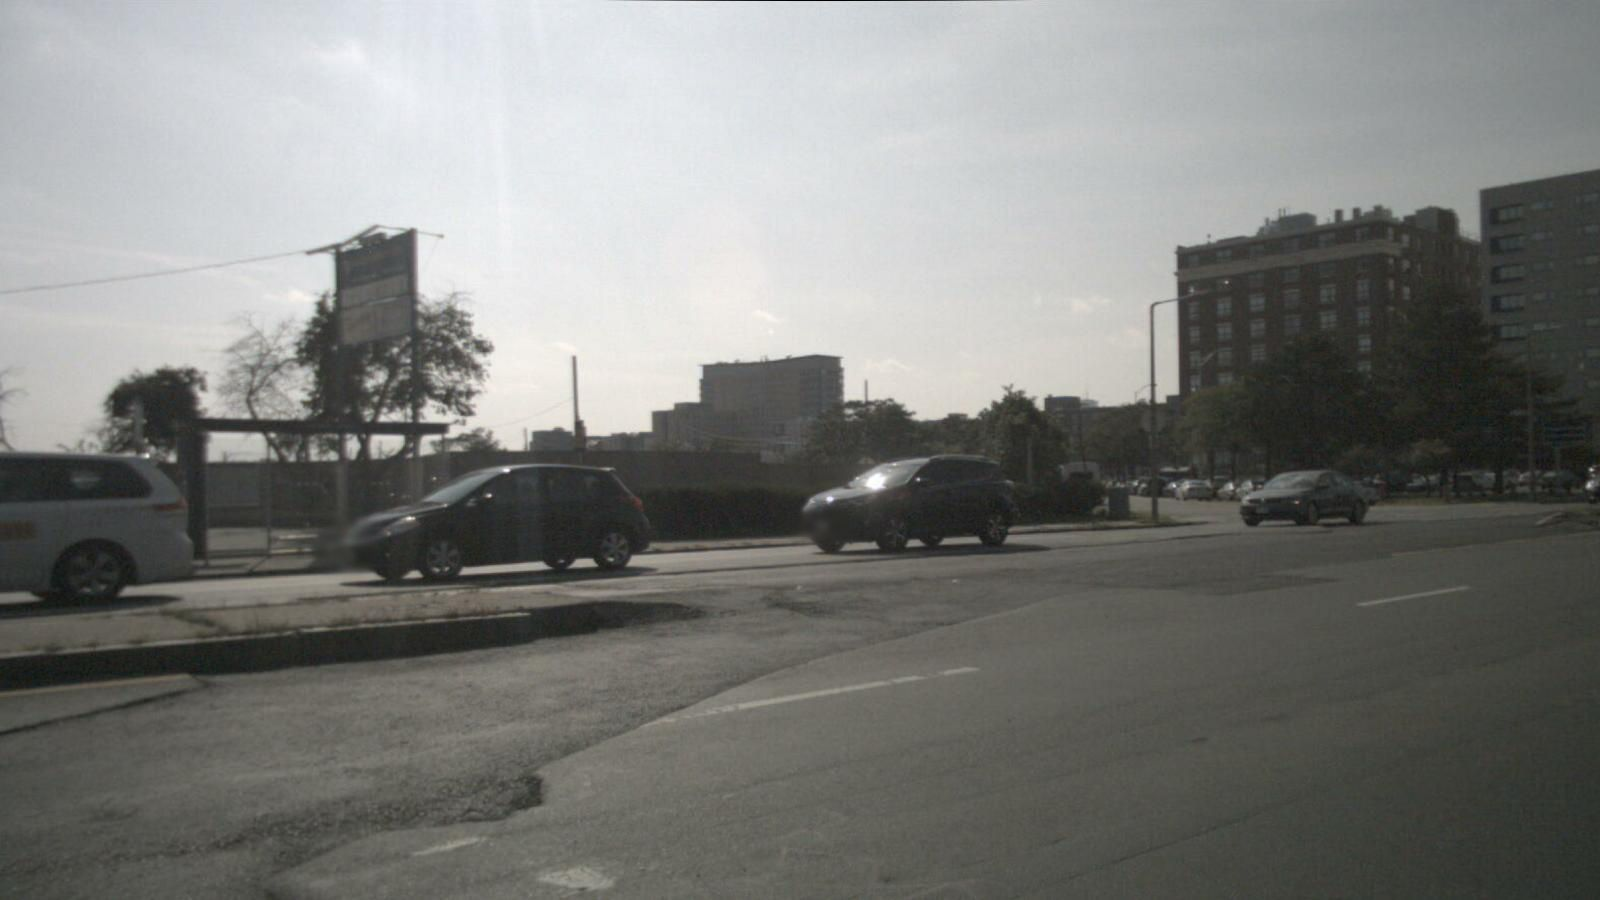
\includegraphics[width=.25\columnwidth, trim={0cm 0cm 0cm 0cm},clip]{fig/optim/optim_input.png}&
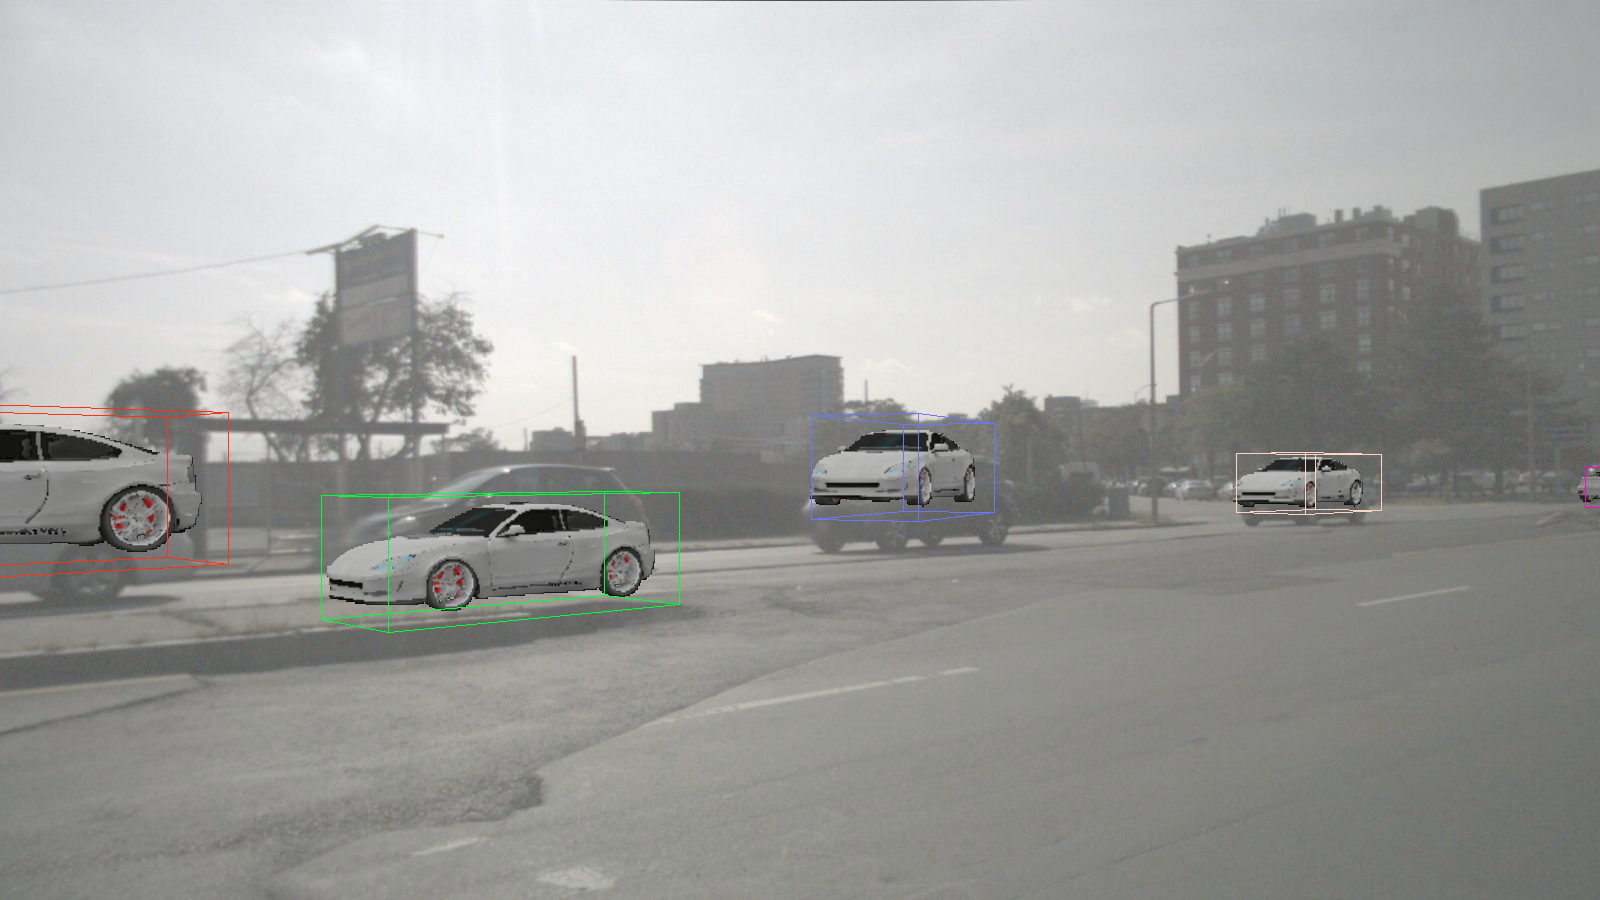
\includegraphics[width=.25\columnwidth, trim={0cm 0cm 0cm 0cm},clip]{fig/optim/init_im_w_bbox.png}&
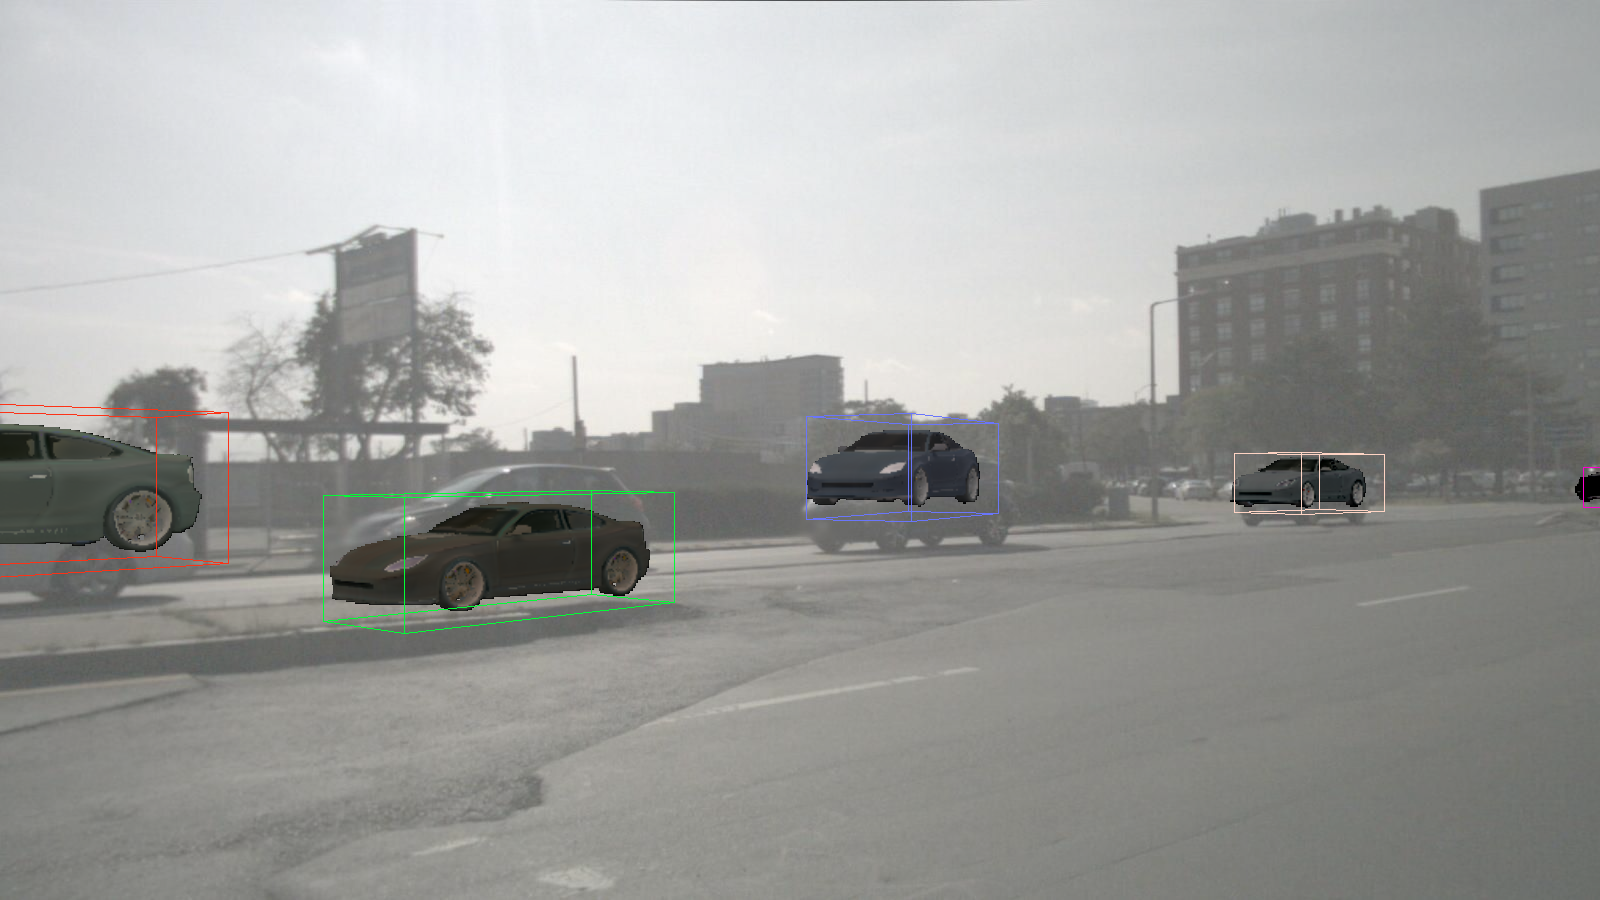
\includegraphics[width=.25\columnwidth, trim={0cm 0cm 0cm 0cm},clip]{fig/optim/texture_im_w_bbox.png}&
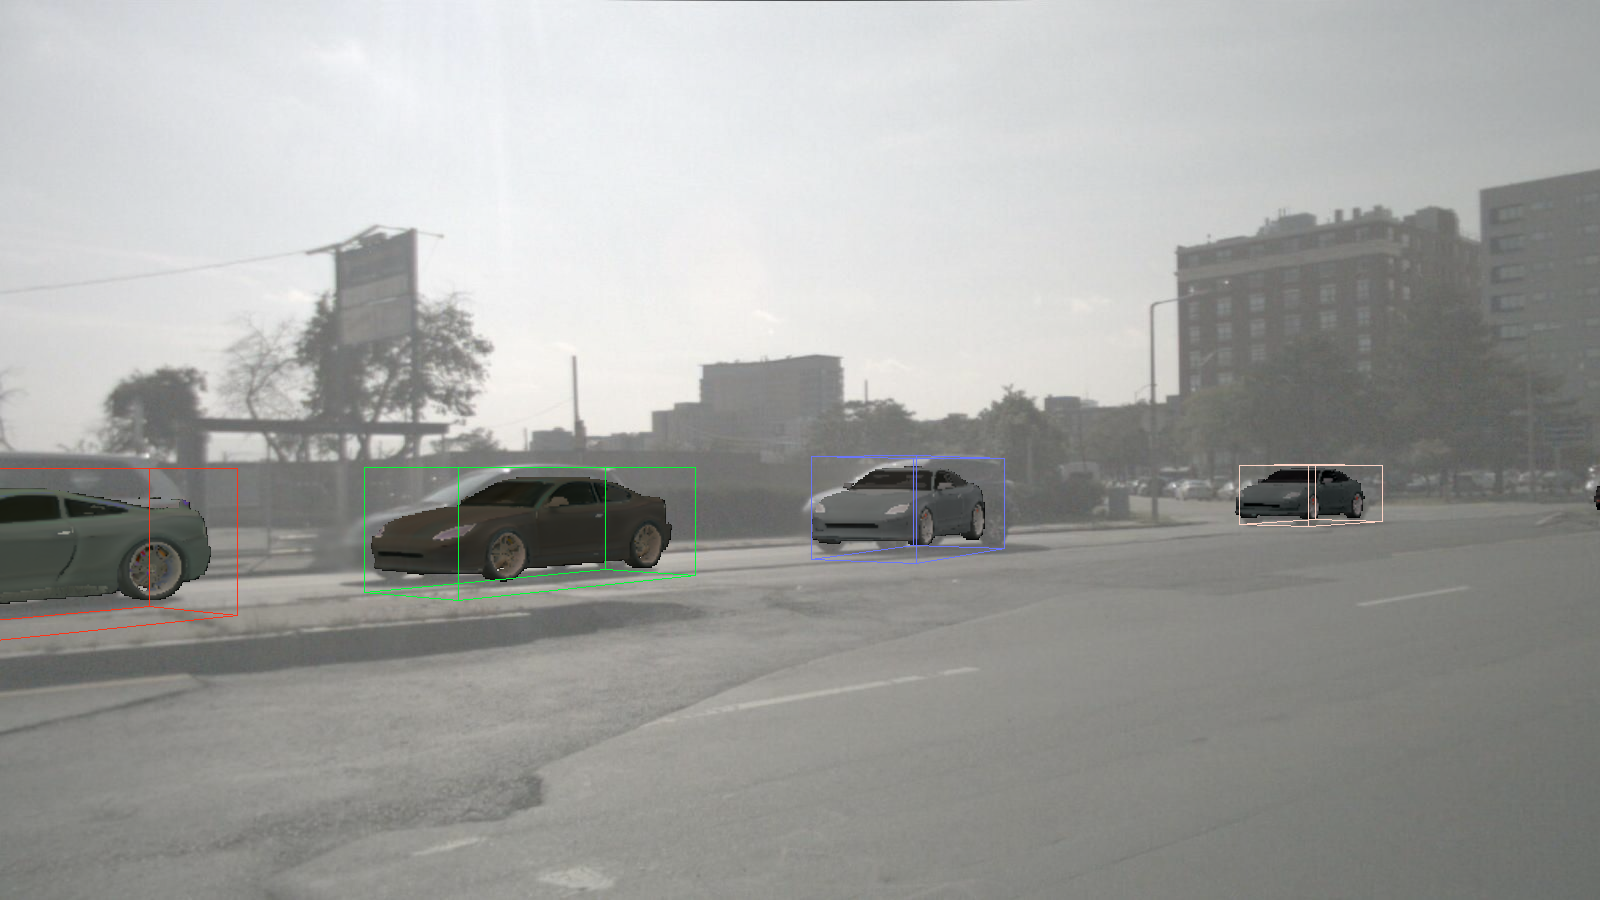
\includegraphics[width=.25\columnwidth, trim={0cm 0cm 0cm 0cm},clip]{fig/optim/pose_im_pil.png}&
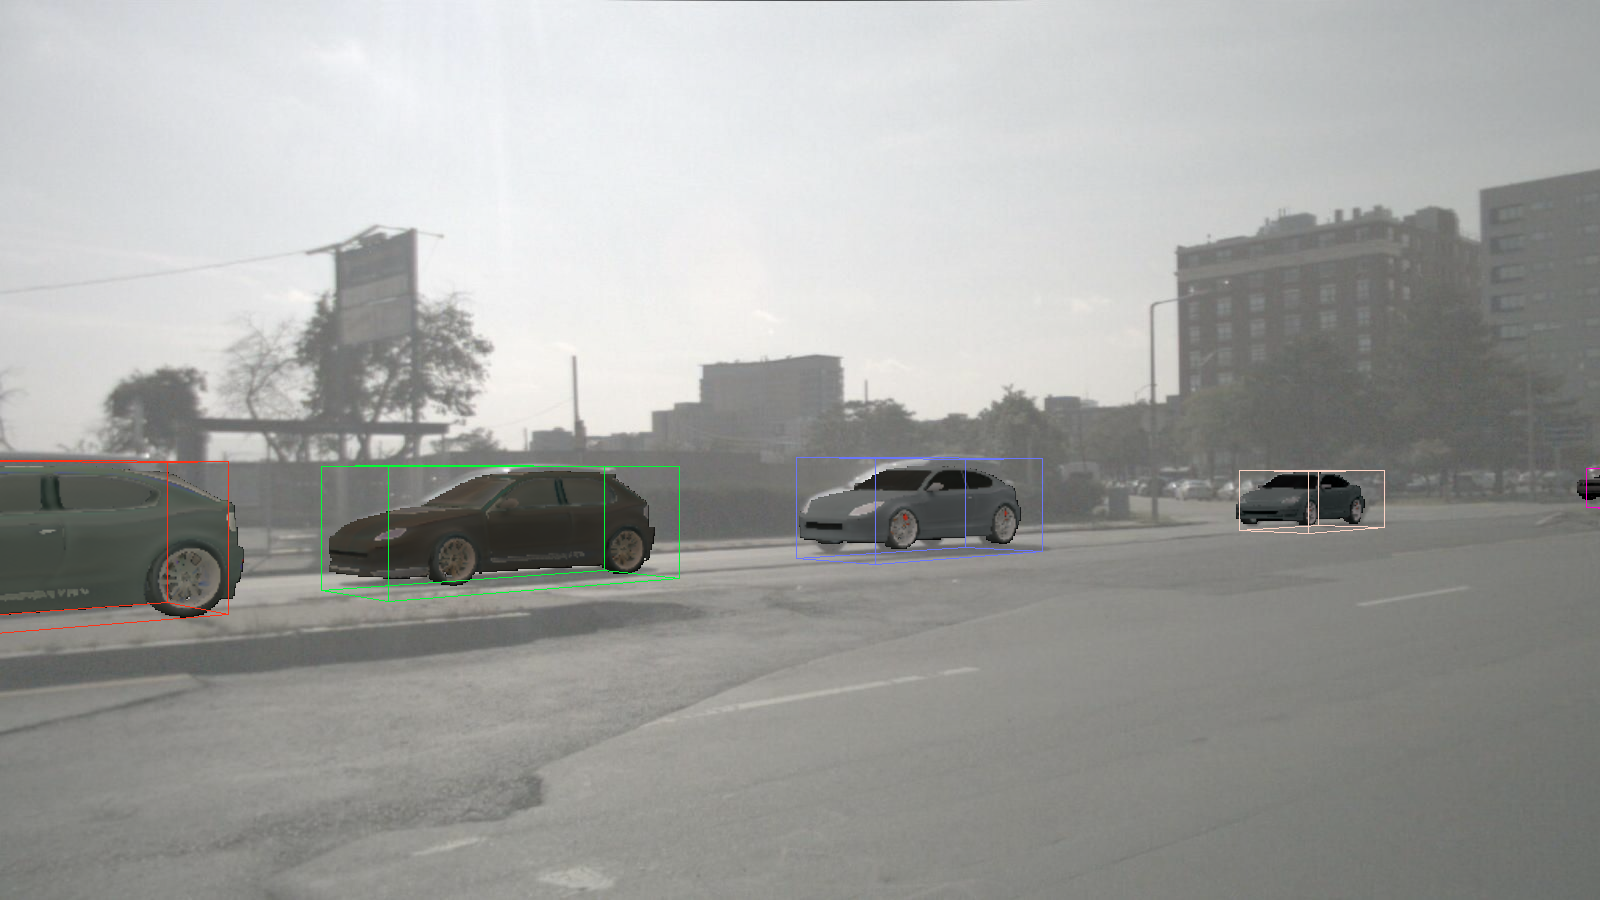
\includegraphics[width=.25\columnwidth, trim={0cm 0cm 0cm 0cm},clip]{fig/optim/final_im_w_bbox.png}\\
& \multicolumn{4}{r}{\textit{Input frame is faded for visibility.}} \\
\end{tabular}}
\vspace*{-6pt} 
\caption{\textbf{Optimization Process.} From left to right, we show (i) the observed image, (ii) the rendering predicted by the initial starting point latent embeddings, 
(iii) the predicted rendered objects after the texture code is optimized (iv) the predicted rendered objects after the translation, scale, and rotation are optimized, and (v) the predicted rendered objects after the shape latent code is optimized. The ground truth images are faded to show our rendered objects clearly. Our method is capable of refining the predicted texture, pose, and shape over several optimization steps, even if initialized with poses or appearance far from the target -- all corrected through inverse rendering.} 
\label{fig:optim}
\vspace*{-16pt}
\end{figure*}
